\section{Leaderboards are Shiny}
\label{ch:isicle:intro}

Leaderboard evaluations---for better or worse---are the
\textit{de facto} standard for measuring progress in question
answering~\citep{squad16} and in many \nlp{}
tasks~\citep{wang2019superglue}.
%
An unfortunate side effect of leaderboard popularity is \abr{sota}-chasing, often at the expense of carefully inspecting data and models~\citep{linzen2020progress}.
For example, the same  ``super-human'' models that top question answering leaderboards~\citep{najberg-18} often fail spectacularly~\citep{feng2018rawr,wallace2019universal} by learning non-generalizable statistical patterns~\citep{mccoy2019heuristics,niven2019probing}.
Finally, focusing \textit{solely} on metrics conflates progress on a specific \emph{task} with progress on real-world \nlp{} \emph{problems} behind the task~\citep{bender2020climbing}.
Plainly, focusing on headline \abr{sota} numbers ``provide(s) limited value for scientific progress absent insight into what drives them'' and where they fail~\citep{lipton2019troubling}.

In this work we take leaderboards ``as they are,'' and imagine how they
might better support research.
%
Leaderboards establish differences between
models on a fixed task.
%
Hence, leaderboards should enable and encourage the comparison of models and
inspection of examples.
%
And leaderboards should also signal when they have outlived their usefulness~\citep{boydgraber2020nerds}.

\begin{figure}[t]
  \centering
  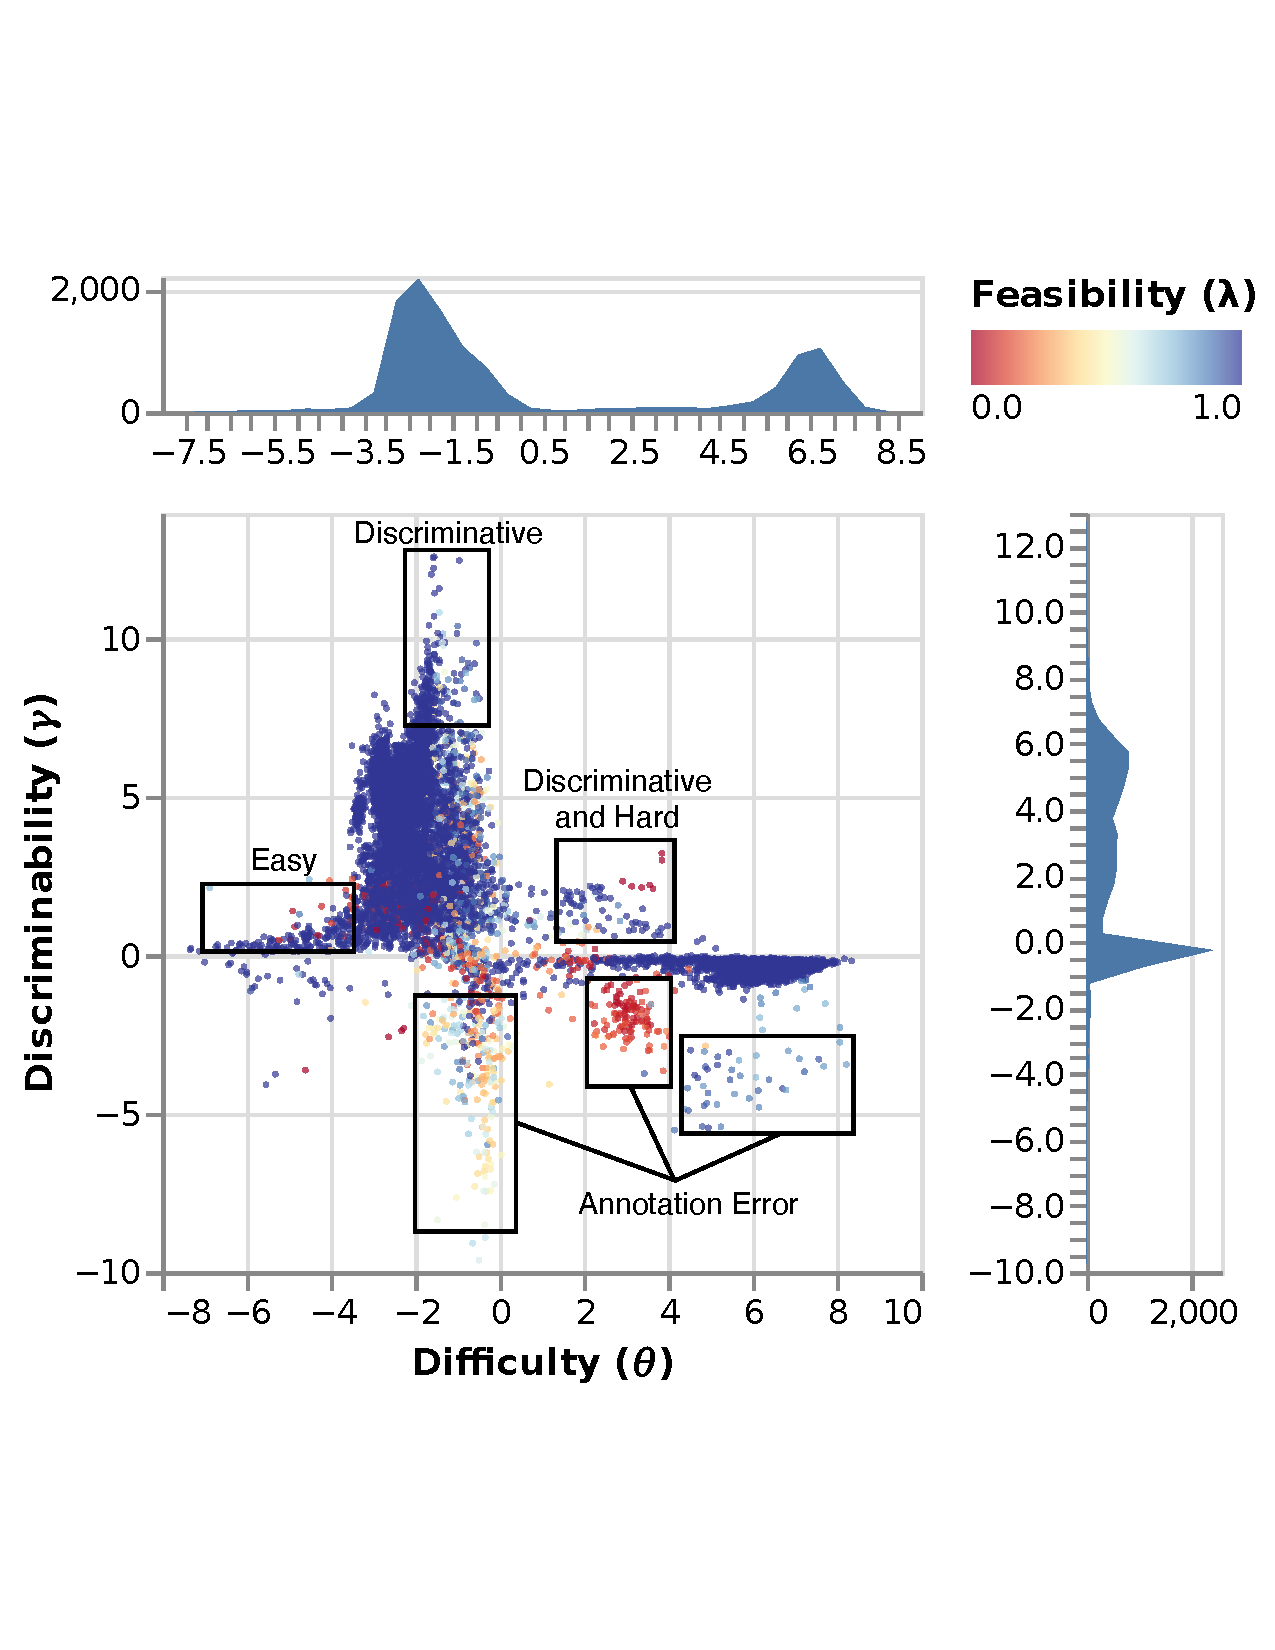
\includegraphics[width=\columnwidth]{annotated_irt_example_dist.pdf}
  \caption{
    Difficulty and Ability Discriminating (\name{}) leaderboards infer the \diff{}, discriminativeness, and feasibility of examples.
    Negative \discability{} suggests an annotation error; for example, the question with most negative \discability{}
    asks ``Why did demand for rentals decrease?'' when the answer is ``demand for higher quality housing increased.''
  }
  \label{fig:irt-dist}
\end{figure}

\subsection{How to Direct Leaderboards' Light}

To help focus attention on examples and models of interest, we propose Difficulty and Ability Discriminating (\name{}) leaderboards that explicitly model both task and submissions \emph{jointly}, rather than either in isolation.\footnote{Source code, data, and visualizations at \projecturl{}.}
%
\name{}'s underlying model is based on Item Response
Theory~\citep[\abr{irt}, reviewed in \S\ref{ch:isicle:lead}]{lord1968test,baker2001irt}, a widely used~\citep{van2016assess} alternative in educational testing to
simple
summary statistics~\citep{edgeworth1888exams}.

\name{} can explicitly identify the \emph{difficulty} and \emph{\discability{}} of \itms{} (Figure~\ref{fig:irt-dist}),\footnote{
  Example and feasibility distribution in Appendix~\ref{ch:isicle:apx:examples}.
  Interactive visualization linked from \href{https://irt.pedro.ai}{http://irt.pedro.ai}.
} which in turn can lead to a more nuanced ranking of models, identifying poor \itms{}, and better understanding of a dataset and task.
%
Throughout the paper, we use the question answering (\qa{}) benchmark \squad{}~2.0~\citep{rajpurkar2018know}.
%
For example, \name{} can identify questions that are challenging to models and questions that are wrong (incorrectly annotated).
%
In addition to better understanding datasets, it is also helpful for
efficiently selecting evaluation items to annotate.
We conclude with recommendations for future leaderboards (\S\ref{ch:isicle:conc}) and discuss where \irt{} in \nlp{} can go next (\S\ref{ch:isicle:future}).
